% 
%  $Author: awl8049 $
%  $Date: 2012/03/16 14:02:50 $
%  $Revision: 1.6 $
%
\documentclass[times, 10pt,twocolumn]{IEEEtran} 
%
% Following stuff is included for page squeezing if we need to cut for 
% a specific conference.   These values are selected from the
% documentation for the savetrees style.  We have to manually set these
% as there is some sort of weird interaction between the IEEE style
% files and the savetrees package that precludes us from directly
% including the savetrees package.
%
% Tigenten up LaTeX's widow control parameters
\let\markeverypar\everypar
\newtoks\everypar
\everypar\markeverypar
\markeverypar{\the\everypar\looseness=-1\relax}
% Float placement
\renewcommand{\topfraction}{0.9}
\renewcommand{\bottomfraction}{0.9}
\renewcommand{\textfraction}{0.1}
\renewcommand{\floatpagefraction}{0.9}
\renewcommand{\dbltopfraction}{0.9}
\renewcommand{\dblfloatpagefraction}{0.9}
\setcounter{topnumber}{50}
\setcounter{bottomnumber}{50}
\setcounter{totalnumber}{50}
\setcounter{dbltopnumber}{50}
% 
% Float spacing
\setlength{\intextsep}{1ex}
\setlength{\floatsep}{1ex}
\setlength{\dblfloatsep}{1ex}
\setlength{\abovecaptionskip}{1ex}
\setlength{\belowcaptionskip}{0ex}
\setlength{\textfloatsep}{1ex}
\setlength{\dbltextfloatsep}{1ex}
%  Reduce interline spacing
\renewcommand{\baselinestretch}{0.9}
% Configure titlesec package to go as tight as possible
\newcommand{\subparagraph}{} % IEEEtran doesn't define, so null it 
\usepackage[tiny,compact]{titlesec}
% Tighten paragraph indentation
\setlength{\parindent}{1em}
% End modifications to try compress space
% Normal stuff for IEEEtran documents...
\usepackage{amsmath,amsthm,amsfonts,amscd} % Some packages to write mathematics.
\usepackage{setspace}
\usepackage{pdfpages}
\usepackage{graphicx}
\DeclareGraphicsExtensions{.png,.jpg,.pdf,.eps}
\graphicspath{{graphics/}}
%\usepackage[caption=false,labelfont=sf,textfont=sf,captionskip=5pt]{subfig}
\usepackage{authblk}
\usepackage{afterpage}
\usepackage{multirow}
\usepackage[section]{placeins}
\usepackage[small]{caption}
\newcommand{\equationname}{Eq.\ }
\newcommand{\equationnames}{Eq.\ }
\newcommand{\figurenames}{Figs.}
\usepackage{titling}
\setlength{\droptitle}{-1cm}
\pretitle{\begin{center}\begin{LARGE}\bf}%
\posttitle{\end{LARGE}\end{center}\vspace{1ex}}%
\preauthor{\begin{center}\begin{large}}%
\postauthor{\end{large}\end{center}}%
\predate{}%
\postdate{}%
\begin{document}
\title{Thermal-Aware Scheduling in  Multicore Systems Using Chaotic
  Attractor Predictors} 
\author{Adam  Lewis} 
\author{Nian-Feng Tzeng} 
\date{}
\affil[]{Center for Advanced Computer Studies, University of Louisiana at
  Lafayette, Louisiana 70504\\
  \{awlewis, tzeng\}@cacs.louisiana.edu }
\maketitle  
\newtheorem{defn}{Definition}
\newtheorem{thm}{Theorem}
\thispagestyle{empty}
\begin{abstract}
  Modern processors crudely manage thermal emergencies through Dynamic
  Thermal Management (DTM), where the processor monitors the die
  temperature and dynamically adjusts the processor voltage and
  frequency (DVFS) to throttle down the processor when
  necessary. However, DVFS tends to yield marked degradation in both
  application performance and system reliability. Thus, pro-active
  scheduling techniques that avoid thermal emergencies are preferable
  over reactive hardware techniques like DTM.  Based on our previously
  introduced thermal Chaotic Attractor Predictors (CAPs), which take into
  account key thermal indicators and system performance metrics for
  overall energy consumption estimation within a given power and thermal
  envelope), we have developed and evaluated an effective thread
  scheduler for multicore systems.  Besides CAPs, our scheduler makes
  use of two basic principles to minimize server energy consumption: (1)
  selecting the thread with the least probability of causing a DTM in
  the subsequent time quantum, for execution on the next available core,
  and (2) migrating execution threads on thermally overextended cores to
  other cool cores via load balancing so as to observe the thermal
  envelope.  Our developed scheduler is evaluated in practice to assess
  its potential advantage resulting from thermal-awareness by
  incorporating CAPs (for temperature prediction) and basic principles
  (for energy reduction) into the existing scheduler in the FreeBSD
  operating system.  Our implemented scheduler is run on a server with
  the Intel Xeon processor for gathering measures of interest (including
  die temperature readings and runtimes) when benchmark codes
  from the PARSEC suite are executed.  The gathered
  results reveal that our proposed scheduler exhibits reduction in mean
  core on-die temperatures by up to 12.8$^{\circ}$C\ while experiencing
  only 1\% to 4\% performance degradation.
\end{abstract}

\section{Introduction}
\label{sec:Introduction}
Modern processors crudely manage thermal emergencies through Dynamic
Thermal Management (DTM), where the processor monitors the die
temperature and dynamically adjusts the processor voltage and frequency
(known as Dynamic Voltage and Frequency Scaling (DVFS)) to throttle down
the processor whenever necessary. However, the use of DVFS tends to
cause significant negative impacts on application performance and system
reliability \cite{Bircher2008,Coskun2008d,Donald2006}. This paper
introduces effective scheduling for preventive thermal management that
minimizes server energy consumption by (1) selecting the subsequent
thread with the smallest thermal impact in the next time quantum to
execute on an available core, and (2) relocating threads run on
thermally overextended cores to other available cores for load
balancing.  As opposed to prior pursuit of thermal-aware scheduling
\cite{Choi2007,Sarood2011,Yang2008} that aimed to bound temperatures
below critical thresholds, our work considers how to schedule high
workload for die temperature management across all cores.

The current generation of operating systems treats those cores in
multicore and virtualized multi-threaded processors (like those with
Intel's HyperThreading technology) as distinct logical units, called
\textit{logical cores}, which are scheduled independently.  However,
dependency and contention exist in shared resources among those logical
cores, and hence they need to be taken into account upon their
scheduling to address performance and energy efficiency. It thus calls
for the need of intelligent, thermal-aware load balancing and scheduling
within the operating system, achievable via modeling full-system energy
consumption based on computational load for effectively predicting
future energy consumption and its associated thermal change.

To this end, we arrive at a thermal model which relates server energy
consumption to the overall thermal envelope, establishing an energy
relationship between workload and overall system thermodynamics.
According to our analysis of experimental measurements of key processor
performance counter readings and performance metrics, it is found that
the measured readings and metrics do not possess linearity and are
\textit{chaotic in nature}.  Hence, our thermal model, based on a
thermal Chaotic Attractor Predictor (tCAP), takes into account key
thermal indicators (like ambient temperatures and die temperatures) and
system performance metrics (like performance counters) for system energy
consumption estimation within a given power and thermal envelope.  This
work demonstrates that effective scheduling can result from taking
advantage of our devised tCAP when dispatching jobs to confine server
power consumption within a given power budget and thermal envelope while
avoiding detrimental impact on thread execution performance.

Dealing with all cores in a multicore system, a thermal-aware thread
scheduler is highly desirable to ensure that all of the cores in such a
system are kept equally busy, realized by migrating threads over all the
cores (no matter whether in the same processors or different ones) when
necessary for load balancing in the system.  Existing schedulers aid in
processor thermal management by dispatching workloads to cores as
tightly as possible within the same processors to expose more
opportunities for power management via shutting down unused cores.
However, computation-bound server workload fully utilizes available
system cores in most times, thereby rendering such schedulers
ineffectual.  Our Thermal-Aware Scheduler (TAS) addresses this problem
by thermally balancing system workload with as little performance
degradation as possible.  

Our TAS is demonstrated and evaluated by adding thermal-awareness to the
existing scheduler in the FreeBSD operating system executed on Intel
Xeon (Woodcrest) processors.  Benchmarks from the PARSEC suite which
represent typical application server workloads, are chosen to evaluate
our TAS.  The gathered results unveil that TAS achieves reduction in
mean core on-die temperatures by up to 12.8$^{\circ}$C\ (from 44.8$^\circ$C
down to 32.0$^\circ$C) under PARSEC benchmarks, while experiencing only
1\% to 4\% performance degradation.  Our TAS compares favorably with a
recent energy-aware scheduling technique \cite{Sarood2011}, which gets
core temperature reduction by up to 4$^\circ$C (from 63$^\circ$C down to
59$^\circ$C) when four parallel scientific applications compatible to PARSEC
benchmarks were executed on a physical 4-core Intel Xeon 5520 processor
(similar to our testbed processor).

\section{Background and Related Work}
\label{sec:related}
Traditional interactive load balancing assumes workload behavior
involves independent tasks that remain quiet for extended periods when
making thread placement decisions.  Server workloads, on the other hand,
are assumed to contain large numbers of threads which are highly
independent of each other and use synchronization objects to ensure
mutual exclusion on small data items.  Modern operating systems make
load balancing more power-aware by placing workloads to cores as tightly
as possible, thereby presenting more opportunities for power management
software to shutdown unused resources.

\subsection{Thermal Modeling}
\label{sec:thermal-modeling}
Existing thermal models all required to fit targeted mathematical
expressions based on time-series observations of temperatures during the
course of executing various workloads.  Expression coefficients were
estimated by minimizing total least square errors between modeling
results and actual temperature readings.  After proper calibration, such
a mathematical expression becomes a model for extrapolating future
temperatures.  Different modeling techniques have been devised using (1)
integer linear programming~\cite{Kursun2009} to meet real-time deadlines
while minimizing hot spots and spatial temperature differentials across
the die, (2) dynamic thermal modeling guided thread migration
~\cite{Gomaa2004}, (3)  priority adjustment of threads assigned to
overheated cores~\cite{Ayoub2011}, or (4) schedule rearrangement
favoring threads that cause the greatest temperature hike while avoiding
DTM events~\cite{Yang2008}. Schedulers based on prior thermal modeling
all rely on readings of hardware performance counters and temperature
sensors.  They can be improved by analyzing on-die thermal variations to
aid in system power and thermal management \cite{Bailis2011}.

However, preceding techniques are reactive to the temperature
approaching the DTM threshold rather than trying to avoid reaching that
temperature in the first place.  A proactive solution with multi-tier
prediction was suggested earlier \cite{Ayoub2011}, where a core level
predictor was employed to convert temperature observations to operating
frequency estimates while a control-theoretic based scheduler was
followed at the socket level for process level scheduling.  Separately,
a scheduling policy was proposed for scheduling memory-bound tasks at slower
frequencies by sorting the tasks in each core's run queue according to
(1) memory intensity, (2) the contribution of each task to the system
power consumption and (3) the current processor
temperature~\cite{Merkel2010}.   Meanwhile, Cool Loop
\cite{Choi2007} and Dimentrodon \cite{Bailis2011} address a lack of heat
slack by inserting additional cycles into the task scheduling to create
thermal slack, naturally leading to performance degradation.  However, such
approaches work ineffectively under many server cases where the slack
in deadlines usually is unavailable.

\subsection{Earlier Scheduling with Load Balancing Support}
\label{sec:therm-comp-workl}
Modern multiprocessor operating systems often take a two-level approach
to task scheduling for maximized system resource utilization. Such an
approach uses a distributed run queue and follows fair scheduling
policies to manage each core at the first level.  Its second level
balances the work load by redistributing tasks across the queues.  Such
two-level schedulers work under three assumptions: (1) threads are
independent, (2) load is governed by queue length, and (3) locality
exists and is important \cite{Hofmeyr2010}.  In practice, however,
common servers often have the following characteristics: (1) their
threads are logically related, with data and control dependencies among
threads, and (2) their threads have equally long life spans
\cite{Hofmeyr2010}, rendering previous two-level scheduling ineffective.

Meanwhile, existing operating systems have made their load balancing
schemes more power-aware by taking advantages of their power management
drivers which intend to find as compact an allocation of processes to
run-queues as possible.  This way presents more opportunities for the
power management software to shutdown unused resources.  Such
power-aware load balancing, while effective for interactive workloads,
works only if system resources are not completely utilized; it becomes
nonviable if the system workload is high (common to high-performance
servers).

\subsection{Chaotic Behavior of Energy Consumption}
\label{sec:chaot-pred-energy}
An analytical model of server energy consumption was built earlier
\cite{Lewis2008,Lewis2010} by modeling energy consumption as a
function of the work done by the system in executing its computational
tasks and of residual thermal energy given off by the system in doing
that work.  The resulting dynamic system expresses energy consumption in
the time domain as follows:
\begin{equation}
  \label{eq:system}
  E_{system}=f(E_{proc},E_{mem},E_{em},E_{board},E_{hdd})
\end{equation}
where each of the terms in the above equation is defined as: (1)
$E_{proc}$: energy consumed in the processor due to computations, (2)
$E_{mem}$: energy consumed in the DDR SDRAM chips, (3) $E_{em}$: energy
taken by the electromechanical components in the system, (4)
$E_{board}$: energy consumed by peripherals that support the operation
of the board, and (5) $E_{hdd}$: energy consumed by the hard disk drive
during the system's operation.

The continuous system in \equationnames~\eqref{eq:system} can be viewed
as a multi-variate differential equation in the time domain that can be
estimated using a time series representation. This time series is
constructed by considering (1) an initial energy state $E_{system}$ at
time $t=0$ and (2) a set of physical predictors that approximate the
values of $E_{proc}$, $E_{mem}$, $E_{board}$, and $E_{hdd}$ at the next
interval $t+\Delta t$.

\newline
\begin{small}
\begin{table}[tbhp]
  \centering
  \caption{PeCs and performance metrics for Intel Xeon server}
  \label{tab:intelmodel}
  \begin{tabular}{l l}
\hline
\hline
\textbf{Variable}&\textbf{Measurement} (for $m$ cores \& $k$ fans)\\
\hline
\hline
\multicolumn{2}{l}{\textit{Application length}}\\
$IR$&Instructions retired \\
\hline
\multicolumn{2}{l}{\textit{Application data set}}\\
$QPL_{P_t}$&Transactions on QPLs between Pair $P_t$ of cores\\
$QPL_{IO}$&Transactions on QPLs for IO Handler\\
$CM_{i}$&Last-level cache misses in  Core $i$, $0\leq i < m$\\
$D_{r}$&Disk bytes read\\
$D_{w}$&Disk bytes written\\
\hline
\multicolumn{2}{l}{\textit{Physical core temperature}}\\
$T_{C_{i}}$&Core $i$ on-die temperature, $0\leq i < m$\\
\hline
\multicolumn{2}{l}{\textit{System temperature}}\\
$T_{A_{j}}$&Ambient temperature sensor $j$, $0\leq j < 3$\\
\hline
\multicolumn{2}{l}{\textit{Electromechanism}}\\
$F_{C_{j}}$&Memory cooling fan $C_j$ speed, $0\leq j < k$\\
\hline
  \end{tabular}
\end{table}
\end{small}
Observations from each time series are measured using (1)~the
appropriate PeCs for the targeted processor (2)~operating system kernel
virtual memory statistics, and (3)~processor die temperatures and
chassis ambient temperatures.  The inputs for our predictor is listed in
Table~\ref{tab:intelmodel}.  They are classified into five groups, each
associated with one server energy contributor.  As one contributor,
application length is estimated in each time period by the quantity
$IR$, the total number of retired instructions of the thread.  Among the
contributor of "application data set" listed in
Table~\ref{tab:intelmodel}, $QPL_{P_{t}}$ and $QPL_{IO}$ are relevant to
QuickPath Links, and they are associated with $E_{proc}$ and $E_{mem}$,
respectively.  Each $CM_{i}$ measures the total last-level cache miss
counts due to Core \textit{i}, $0 \leq i$ < $m$, $m$ being the number
of cores in the processor, and they determine $E_{mem}$.  As the
contributor of "physical core temperature," the core die temperature
measures are pertinent to $E_{proc}$.  The subsequent measures dictate
$E_{board}$, obtained from 3 temperature sensors placed on the board for
ambient temperature readings and Finally, $F_{C_{j}}$ measures speed
information of those nine memory cooling fans which determines $E_{em}$.

\subsection{Limitations of Existing Scheduling}
\label{sec:shortc-comp-workl}
Current power management software that utilizes DVFS techniques to
address DTM events has been effective in addressing thermal emergencies
\cite{Donald2006,Hanson2007}, commonly implemented in modern server
processors.  However, handling DTM through DVFS
can be problematic due to issues with program phase behavior and
contention for shared resources \cite{Bircher2008,Coskun2008d},
resulting directly from slow transitions between the active and the idle
device states and also from inability to access resources associated
with idle processors.  When the power phase changes frequently, abundant
thermal variations among cores within the processor occurs, leading to
decreased reliability \cite{Coskun2008d,Kursun2009}.

A study of OS-level thermal migration using Linux on the IBM POWER5
processor~\cite{Choi2007} discovered that the rise and fall times of
core temperatures vary in the order of hundreds of milliseconds.  As
most operating systems choose scheduler ticks to be of 10 ms or less, it
often is impossible to react to thermal conditions before a critical
state is reached.  As a result, three improvement mechanisms for
managing thermal states have been pursued: (1) core hopping for
leveraging spatial heat slack, (2) task scheduling for leveraging
temporal heat slack, and (3) SMT scheduling for leveraging temporal heat
slack.  In the presence of slack, each of those mechanisms may reduce
core die temperatures by 3 to 5$^{\circ}$ C on an average, at the
expense of 3\% mean performance degradation ~\cite{Choi2007,Ayoub2011}.
However, in the absence of slack commonly found under heavy workloads in
high-performance servers, the three mechanisms becomes ineffective,
calling for suitable scheduling with thermal awareness proactively.

\section{Proposed Thermal Aware Scheduler}
\label{sec:sdesign} 
The scheduler in an operating system is responsible for making two
decisions in each time quantum: (1) thread scheduling, i.e., deciding
the next thread to run on an available core and (2) load balancing,
namely, distributing workload evenly across all cores, with existing
implementations mostly focusing on performance.  Our TAS (Thermal Aware
Scheduler) incorporates a heuristic scheduling algorithm in a popular
scheduler (i.e., ULE in the FreeBSD operating system) for thermal stress
reduction on a multicore processor while meeting the SPMD requirements
of equal execution progress and maximum parallelism exploitation.

\subsection{Thermal Predictors}
\label{sec:therm-pred-design} 
An application $A$ is composed of $p$ execution threads, with a data set
$D_{A}$ consisting of $d_{i}$ data per processor, for $1\leq i \leq
p$. Thus, energy consumed by executing application $A$ with data set
$D_{A}$ can be expressed as:
\begin{equation}
\label{eq:eworkload} 
E_{A}(A,D_{A},t) = \displaystyle \sum_{i=1}^{p}W(\tau_{i},d_{i},t_{i})
\end{equation}
for $1\leq i \leq p$, where $W$ is the workload associated with
execution thread $\tau_{i}$ involved in application $A$, $d_{i}$ is the
corresponding data set for that thread, and $t_{i}$ is its thread
execution time.  The workload $W$ is measured in terms of the number of
bytes operated upon or transferred over, during the course of completing
those instructions retired by the logical core for each thread $p$. We 
relate system energy expenditure (upon application execution)
to corresponding joule heating by defining ``Thermal Equivalent of
Application'' (TEA) as the electrical work converted to heat in running
the application, leading to die temperature change and ambient
temperature change of the system:
\begin{equation}
\label{eq:tea} \Theta(A, D_{A}, T, t) =
\frac{E_{A}(A, D_{A}, t)}{\displaystyle \lim_{T \to T_{th}} J_e(D_{A}, \Psi_{cp}) (T -T_{nominal})},
\end{equation} 
where $T_{th}$ denotes the threshold temperature at which a thermal
emergency event will occur, and $T_{nominal}$ refers to the nominal
temperature as reported by the system when the operating system is
running without any application execution.  The term $J_{e}$ is the
``electrical equivalent of heat'' for the chip, which reflects the
processing the data bits during application execution and the black
body thermal properties of the chip packaging as well as the cooling
mechanisms around the chip, as defined by the parameter $\Psi_{cp}$.
The value of $\Psi_{cp}$ is an ambient thermal characterization
parameter provided by the hardware manufacturer to relate temperature to
power for cooling purposes~\cite{Intel2006}.   We compute the 
the into achieved performance per unit energy consumed by the
chip:
\begin{equation}
\label{eq:thermcost} 
C_{\theta}(A, D_{A}, T, t)=\frac{\Theta (A, D_{A}, t)}{E_{A}(A, D_{A}, t)}
\end{equation}
This normalized quantity indicates the ``cost'' of executing an
application on a given processor, with $E_{A}(A, D_{A}, t)$ obtained
from energy consumption of individual physical components (processor,
DRAM units, HDD, motherboard, and electrical/electromechanism) given by
\equationname~\eqref{eq:system}.

Following the procedure reviewed in Section~\ref{sec:chaot-pred-energy}
(and detailed in \cite{Lewis2010}), we create thermal Chaotic Attractor
Predictors (tCAP) for $\Theta$ and $C_{\theta}$ as a means for
predicting the thermal behavior during application execution.  We
enhance the existing FreeBSD operating system to maintain information
required by the thermal estimator.  Our design is based on the
concept of Task Activity Vectors (TAVs) introduced earlier
\cite{Merkel2008a}, with a vector for each kernel thread to store the
required history in order to make sound prediction.  Generally, the more
additional space is employed for history maintenance, the higher benefit
our thermal scheduling gains.

\begin{figure}[btph] \centering
  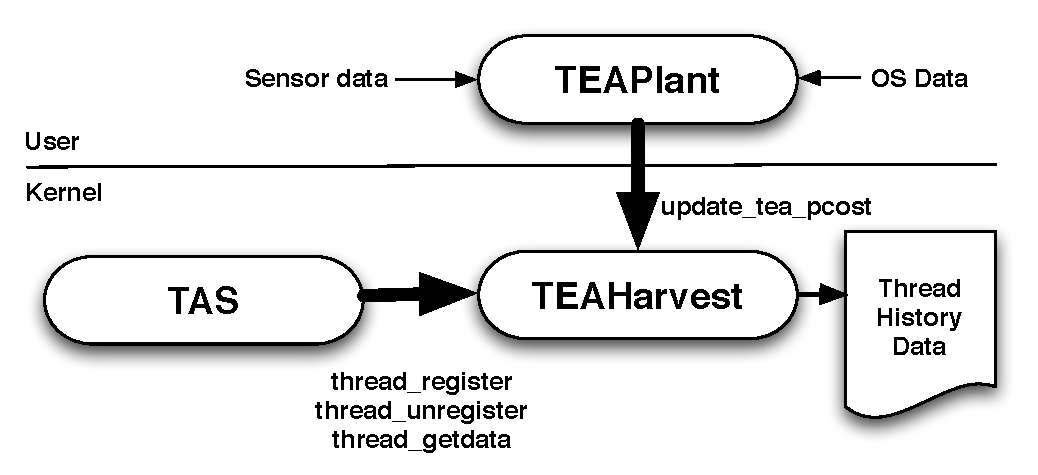
\includegraphics[scale=0.45]{tasdesign}
  \caption{TEAPlant and TEAHarvest data collection.}
  \label{fig:teaplant}
\end{figure}
The high-level design of TAS is shown in
\figurename~\ref{fig:teaplant}. A user-level daemon process collects
required information to compute the tCAP predictions. Temperature
readings are collected by this process from the digital temperature
sensor associated with a core.  Similarly, processor performance
counters are gathered by the same process, with both sets of metrics
used to generate estimates. Estimates are posted via a system call
interface to a device driver that collects the data for use by the
currently executing thread.  The scheduler queries this driver via a
kernel function call interface when making scheduling decisions to
determine the $\Theta$ and $C_{\theta}$ estimates associated with a
thread.

\subsection{Thread Scheduling}
\label{sec:selection} 
The scheduler uses the cost predictor for $C_{\theta}$ to predict a
thread's impact on core temperature and adjust the
thread priority as required to prevent an increase in core temperature.
TAS maintains three queue structures per core: an idle queue, a
current queue, and the next queue. The core executes all work on the
current queue and then swaps its current queue and its next queue. For
performance reasons, our implementation follows the convention used by
the existing FreeBSD ULE scheduler, placing real-time and interrupt
threads on the current queue.  This is a reasonable limitation given that
real-time thread deadlines must be satisfied and 
interrupt service routines are typically short in length.

All other threads are scheduled in terms of an interactivity score.  As
with the ULE scheduler, the interactivity of a process is
determined by the formula of
\begin{equation}
\label{eq:interactsleeprun} 
I =   
\begin{cases}
  S / (SL/RUN) & \text{if sleep time} \geq \text{run time}\\
  (S/ (SL / RUN))+S & \text{if run time} < \text{sleep time}
\end{cases}
\end{equation}
where $I$ is the interactivity score, $S$, the scaling factor of the
maximum interactivity score divided by two, and $SL$ and $RUN$ refer
respectively to the cumulative sleep and run times for the thread.   
Threads whose scores fall below a predefined threshold are considered
interactive and are assigned to the current queue, while all other
threads are assigned to the next queue.

For our TAS, the interactivity score $I$ is scaled by the predicted
value of $C_{\theta}$, normalized to a percentage value.  It was shown
previously \cite{Zhou2010b} that the greatest thermal benefit occurred
when a scheduler favored the thread which moved the core temperature as
close as possible to the DTM threshold without actually triggering a DTM
event.  TAS achieves a similar effect by scaling the interactivity of a
thread its normalized execution cost, thereby giving less ``thermally
costly'' threads greater opportunities for execution so as to moderate
the processor temperature.  Penalizing more thermally costly threads
reduces the opportunities for such threads to gain access to logical
cores, presenting similar advantages of techniques which artificially
inject slack into thread scheduling but without extra scheduling
overhead incurred to those techniques.

\subsection{Load Balancing}
\label{sec:loadbalance} 
Load balancing distributes workload evenly across the available logical
cores, with current implementation mostly aiming to maximize
performance.  This work applies load balancing to minimize thermal
stress while seeking best performance.  Specifically, TAS organizes
system cores into ``thermal clans'' based upon the temperature and
execution frequency.  Specifically, a local core is assigned to one of
the three thermal clans: Hot, Warm, and Cold, if its on-die temperature
is respectively 90\% or higher, between 75\% and 90\%, and below 75\% of
the DTM threshold temperature.  Note that if a physical core supports
$\alpha$ threads, $\alpha$ logical cores will result from the physical
core, with their temperatures all equal to that of the physical core.
In addition, logical cores are grouped into fast and slow clans
according to the execution frequencies of their underlying physical
cores.  This two-level categorization allows TAS to manage work load
distribution better from the thermal and performance prospectives, by
migrating work away from hot units with negligible execution performance
degradation.

For performance reasons, information about thermal clans of all logical
cores is maintained by the TEAHarvest thermal predictor driver.  The
driver allocates threads to local cores for execution, according to
thermal efficiency and cost estimates.  TAS scheduler queries the driver
to determine whether a core will move towards the DTM threshold
temperature if a thread becomes ready to execute on one of its logical
core.  In this way, TAS predicts whether a thread moves its assigned
core closer to a DTM event and adjusts the core's run-queue accordingly
to prevent DTM occurrence.

On a periodic basis (i.e., once in every 500 ms), the TAS scheduler
balances the workload among logical cores, giving sufficient times for
overtaxed resources to thermally recover.  For each thread in the run
queue, TAS uses the tCAP to estimate the value of $\Theta$ for each
thread in the queue and predict the resulting change in temperature if
this thread were to execute.  It then moves the thread with the greatest
temperature impact to the least loaded logical core in the ``Cold''
clan.  This way results in workloads being moved away from thermally
stressed logical cores, while maintaining execution performance.

Periodically, the system reads the temperatures of it all logical cores
and, if required, also moves a logical cores to a different thermal
clan.  It should be noted that the time required for a logical core to
recover from a thermal event is significantly longer than the interval
used for thread scheduling~\cite{Choi2007}. This allows our TAS to use a
much larger interval (2 seconds) between scans (across core
temperatures) to determine if any logical core must be assigned to a new
thermal clan for better scheduling outcomes.

\section{Experimental Evaluation and Results}
\label{sec:experiment} 
We have evaluated our TAS (Thermal Aware Scheduler) using the FreeBSD
operating system run on a commodity server.  Our TAS implementation
modified the existing thread selection and load balancing in FreeBSD's ULE
scheduler~\cite{McKusick2004} to take into account both thermal behavior
and system performance, as elaborated in Section~\ref{sec:sdesign}.  PeC
data were collected at the user level through standard tools provided
for the data collection purpose by FreeBSD (i.e., the \texttt{coretemp}
and \texttt{hwpmc} kernel extensions).  They were collected and collated
by a FreeBSD kernel extension, made available to the operating system
scheduler for query when making scheduling decisions
(\figurename~\ref{fig:teaplant})

The processor thermal model was calibrated by measuring behavior
outcomes of the testbed with TAS at idle and under high load stress
using common utilities from the FreeBSD regression test suites and
software collections.  Benchmarks from the Princeton Application
Repository for Shared-Memory Computers (PARSEC) suite~\cite{Bienia2011}
were then evaluated on the testbed to assess TAS in terms of key metrics
of interest (i.e., die temperature, benchmark runtime, and mean power dissipation)
under high parallelism in the thread level.

\begin{small}
\begin{table}[tbhp] 
\centering
  \caption{Processor used in evaluation}
  \label{tab:hardware}
  \begin{tabular}{l l} 
\hline 
\hline
&\textbf{Dell Precision 490}\\ 
\hline 
CPU&Intel Xeon 5300 (Woodcrest)\\ 
CPU L2 cache&4MB\\ 
Memory&8GB, DDR2 667Mhz with ECC\\
Internal disk&500GB\\ 
Network&1x1000Mbps\\ 
Video&NVIDA Quadro FX3400\\ 
\hline
  \end{tabular}
\end{table}
\end{small}
\subsection{Experiment Setup}
\label{sec:experiment-setup} 
Experimental evaluation was conducted on our testbed running TAS, with
its hardware specified in Table~\ref{tab:hardware}.  The key metrics of
interest were gathered during the course of application execution.
Power dissipated was measured by a WattsUP power meter
\cite{WattsUp2006a}, connected between the AC Main and the server
testbed.  The power meter measured the total and average wattage,
voltage, and amperage over the run of a workload.  The internal memory
of the power meter was cleared at the start of each run and the measures
collected during the runs were downloaded (after execution completion)
from the meter's internal memory into a spreadsheet.

\subsection{tCAP Establishment}
\label{sec:callibration}
Since our TAS relies on tCAP (thermal Chaotic Attractor Predictor) of
the testbed for effectively predicting its thermal behavior during
application execution, it is required first to establish tCAP using
suitable applications.  Two applications were employed as training
applications for deciding the coefficients of the chaotic attractor
predictor: the idle scenario and the most stress scenario.  An idle
application referred to no application thread ready for execution and
thus the testbed runs only the OS threads, whereas the most stress
application leads to the highest processor utilization coupled with
heaviest memory activities, achieved by launching multiple instances of
the FreeBSD \texttt{cpuburn} stress testing codes for concurrent
execution, one per core with symmetric multiple threads disabled.  The
\texttt{cpuburn} stress test code implements a single-threaded infinite
loop with a sequence of integer and floating-point operations and large
blocks of memory reads and writes to thermally stress the testbed
system, driving it close to a thermal emergency.  These two extreme
thermal scenarios is effective for tCAP establishment because any
typical application execution will lie between the two extremes, as far
as the coefficients of tCAP are concerned.

These two training scenarios run for 600 seconds, with PeCs sampled at
an interval of $t=5$ seconds for establishing tCAP.  The procedure for
tCAP establishment is the same as what was described earlier
\cite{Lewis2010}, and it involved three steps. First, the training set
is constructed by consolidating the observed PeCs into a time series
using geometric means.  In the second step, the Takens Embedding
Theorem~\cite{Su2010} is applied to find delay embedding, with the
nearest neighbors algorithm then employed to identify the set of
attractors using the embedded set.  Finally, our tCAP is established by
solving the linear least squares problem resulted from fitting a
multi-variate polynomial to the attractor set.  The time complexity of
establishing tCAP equals O($n ^2$), where $n$ is the number of sampled
PeCs~\cite{Lewis2010}.  Note that the establishment of the attractor set
for tCAP is required only once for a processor type, irrespective of
applications executed on the processor.

\begin{small}
\begin{table}[phbt] 
\centering
 \caption{PARSEC benchmarks used in evaluation}
\label{tab:parsecbench}
\begin{tabular}[bthp]{l l p{5cm}} 
\hline 
\hline 
bodytrack &  & Computer vision image tracking application \\
canneal &  & Simulated annealing chip routing cost computation \\
facesim &  & Physical simulation of facial behavior \\
ferret &  & Content-based similarity search \\
freqmine &  & Simulate FP-growth method for Frequent Itemset Mining \\
streamcluster &  & Online clustering algorithm for data mining \\
swaptions &  & Simulated pricing of portfolio options \\
\hline
\end{tabular}
\end{table}
\end{small}
\subsection{PARSEC Benchmark Results and Discussion}
\label{sec:mult-behav} 
Selected benchmarks from the PARSEC~\cite{Bienia2011} suite, described
in Table~\ref{tab:parsecbench}, were used to evaluate our TAS.
They were compiled with the POSIX \texttt{pthreads} library and executed
using the PARSEC \texttt{native} input sets.  Being parallel workloads
selected from the fields of computer vision, computational finance,
enterprise servers, and animation physics, PARSEC
benchmarks represent real life applications that 
can benefit markedly from scheduling their abundant independent threads
freely based on thermal prediction.

\begin{figure}[tbp] 
\centering
  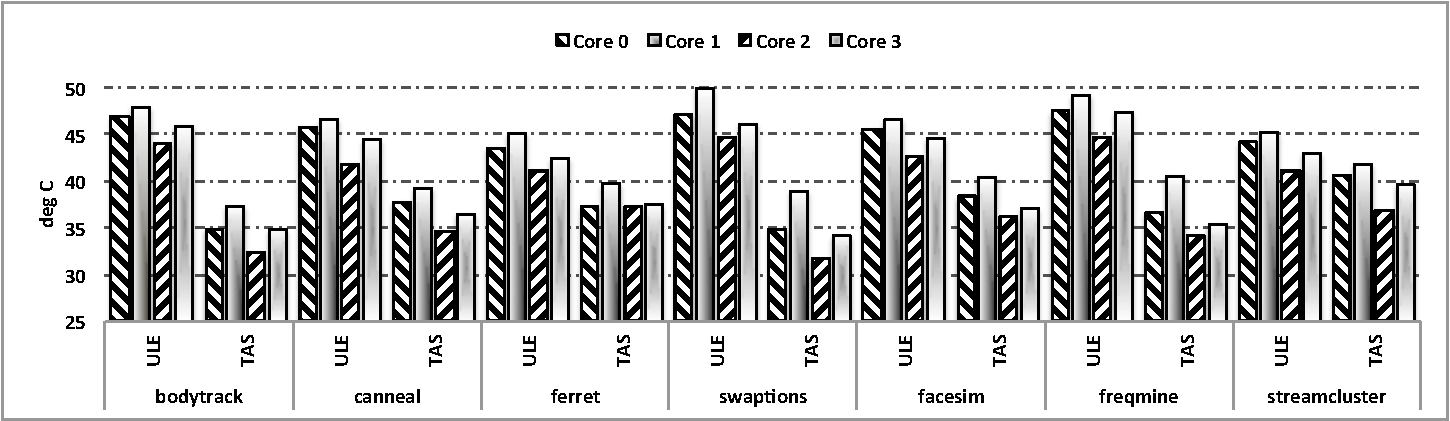
\includegraphics[width=1.0\linewidth,height=1.7in]{graphics/parsectemp}
  \caption{Comparison of PARSEC benchmark average core die temperatures
under ULE and TAS schedulers.}
  \label{fig:pbenchmarkt}
\end{figure}
\begin{figure}[tbp]
  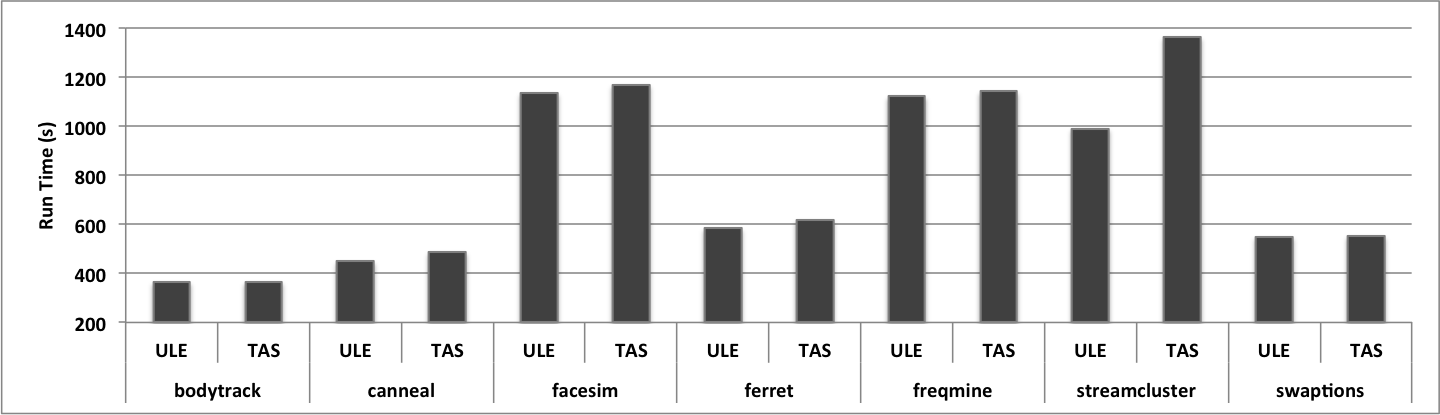
\includegraphics[width=1.0\linewidth,height=1.3in]{graphics/parsecperformance}
  \caption{Comparison of PARSEC benchmark performance under ULE and TAS
schedulers.}
  \label{fig:pbenchmarkp}
\end{figure} 
Three behavior metrics of interest under TAS are gathered: (1) the
average core on-die temperature, (2) the benchmark run time, and (3)
mean system power dissipation.  The outcomes of average core on-die
temperatures upon executing those seven PARSEC benchmarks are depicted
in \figurename~\ref{fig:pbenchmarkt}.  As can be seen from the figure,
the core on-die temperatures range from 32$^\circ$C (for the
\texttt{swaption} benchmark) to 42$^\circ$C (for the
\texttt{streamcluster} benchmark)
under TAS, with \texttt{swaption} and \texttt{bodytrack} (or
\texttt{streamcluster}) experiencing the lowest (or highest) mean
temperature across the four cores.  Temperature outcomes for the same
benchmarks under the classical ULE scheduler are also included in
\figurename~\ref{fig:pbenchmarkt} for comparison.  It is found that
temperature reduction amounts are larger for benchmarks with smaller
working sets (like \texttt{bodytrack} and \texttt{swaptions}).  This is
because such a benchmark has a lower cache requirement \cite{Bienia2011}
and thereby lets TAS schedule threads more freely according to thermal
prediction with negligible performance degradation, resulting in better
temperature reduction.  Consequently, TAS enjoys temperature reduction
by up to 12.8$^{\circ}$C (from 44.8$^{\circ}$C down to
32.0$^{\circ}$C) for the \texttt{swaptions} benchmark.
  
Benchmarks with streaming functions, such as \texttt{facesim},
\texttt{freqmine}, and \texttt{streamcluster}, all have large working
sets, which hinder TAS from scheduling threads freely based on thermal
prediction, since doing so degrades performance considerably.  Hence,
those benchmarks tend to yield less temperature reduction under TAS,
with the average core on-die temperature lowered by 3-6$^{\circ}$C.  

Execution performance (measured in terms of the benchmark runtime) under
TAS is depicted in \figurename~\ref{fig:pbenchmarkp}.  When compared
with the runtime results under ULE included in the figure, it can be
observed that TAS leads to negligible performance degradation, by no
more than 3.3\% for all benchmarks examined except
\texttt{streamcluster}.  Considerable performance degradation is seen
for the \texttt{streamcluster} benchmark, however, likely due to its high
computational intensity as the data set grows with rising dimensionality
and thereby calling for more synchronization required.  As a result, TAS
experiences noticeable performance degradation when scheduling threads
based on thermal prediction.

Mean system power dissipation for each of the PARSEC benchmarks run on
our testbed under both schedulers is shown in
\figurename~\ref{fig:pbenchmark}.  When compared with ULE, TAS is
observed to reduce power dissipation markedly, from 14W (for the 
\texttt{ferret} benchmark) to 19W (for \texttt{swaptions}), due to their
relatively small working sets.  On the other hand, less reduction in
power dissipation is found for benchmarks with large working sets,
lowering power by the range of 3W (for \texttt{streamcluster} to 10W
(for \texttt{facesim}).
  
\begin{figure}[tbp]
  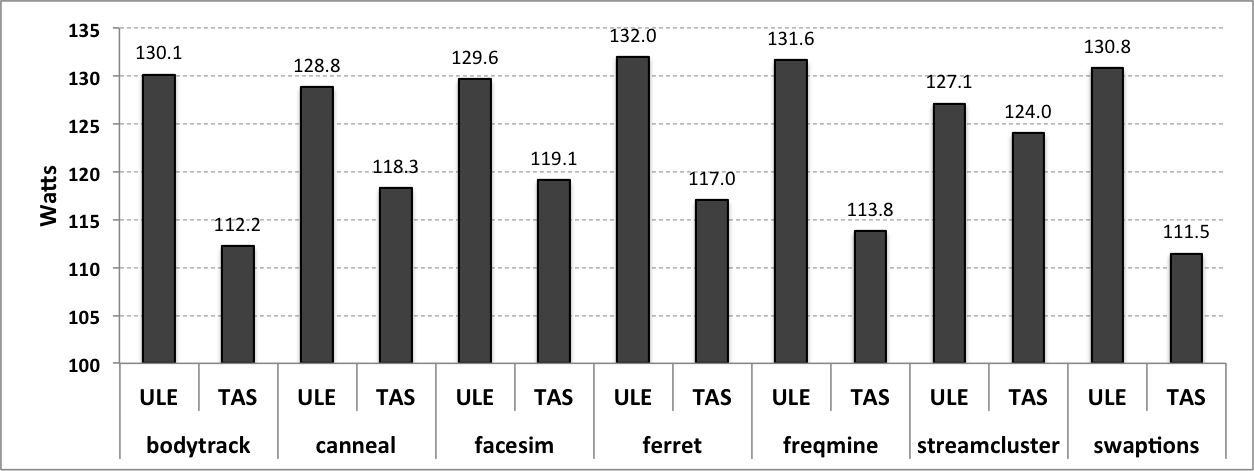
\includegraphics[width=1.0\linewidth,height=1.3in]{ParsecPowerConsumption.png}
  \caption{Comparison of PARSEC benchmark average power dissipation under ULE and TAS schedulers.}
  \label{fig:pbenchmark}
\end{figure}

\section{Conclusion}
\label{sec:conclusion}
Dense servers pose power and thermal challenges, which often cannot be
addressed satisfactorily by conventional DVFS and DTM mechanisms,
especially under heavy workloads common for high-performance systems.
We have investigated into thermal-aware scheduling to deal with such
challenges, capable of managing system energy consumption within a given
power and thermal envelope effectively.  As opposed to prior work aiming
to bound temperatures below critical thresholds, our proposed scheduler
considers how to dispatch heavy workloads in the high-performance
multi-core system for die temperature management across all cores.  It
is based on the thermal Chaotic Attractor Predictors (tCAPs) we develop
to guide thread selection and load balancing, taking into account key
thermal indicators and system performance metrics for preventing DTM
instances proactively.  The proposed tCAP-oriented scheduling (dubbed
the TAS scheduler) has been implemented to augment the original
scheduler of the FreeBSD operating system (called the ULE scheduler) for
evaluation on a testbed server under benchmarks from the PARSEC suite.
Experimental results demonstrate that our TAS scheduler can lower the
mean on-die core temperature by up to 12.8$^{\circ}$C (from 44.8$^\circ$C
down to 32.0$^\circ$C), in comparison to the ULE
scheduler.  When compared with a recent energy-aware scheduling
technique reported to attain core temperature reduction by up to
4$^\circ$C (from 63$^\circ$C down to 59$^\circ$C) upon executing four
parallel scientific applications compatible to PARSEC benchmarks on an
Intel Xeon 5520 4-core processor \cite{Sarood2011}, our TAS clearly
enjoys better thermal reduction under multi-threaded execution.

\label{sec:references}
\begin{small}
\bibliographystyle{savetrees}
\bibliography{../overall.bib}
\end{small}
\end{document}
% The following comment block is used by the different flavors of EMACS and
% the AUCTEX package to manage multiple documents.  In order for AUCTEX
% to understand you're working with multiple files, you should define
% the TeX-master variable as a file local variable that identifies your
% master document.
%
% Please do not remove.
%%% Local Variables: 
%%% mode: latex
%%% TeX-master: "weed2012.tex"
%%% TeX-PDF-mode: t
%%% TeX-source-correlate-mode: t
%%% End: 
